\documentclass[addpoints]{physlabs}

\labtitle{Coulomb's Law}
\labnum{6}
\labnumroman{VI}
\course{PHYSICS 114 - 122 - 182}
\coursesubtitle{General Physics II and Electricity \& Magnetism}
\date{\today}

\begin{document}

\maketitle

% PRELAB SECTION
\begin{prelab}

    \question[1] Why is it important to recharge the spheres before each measurement?
    \begin{solution}[1cm]
    \end{solution}

    \question[2] Compute the force between one gram of protons and one gram of electrons that are $10$km apart.
    Show your work and explain your steps.
    \begin{solution}[2.5cm]
    \end{solution}

    \question[3] Consider the function $y=x^n$ when $n=-2$.
    Fill out the table on the left for the given values of $x$.
    Plot $\ln x$ vs. $\ln y$ on the right.
    Make sure you draw your coordinate axes in a smart way.
    Explain how to obtain $n$ from the graph (Hint: can you fit a straight line to your plotted points?).\\
    \vspace{5pt}\\
    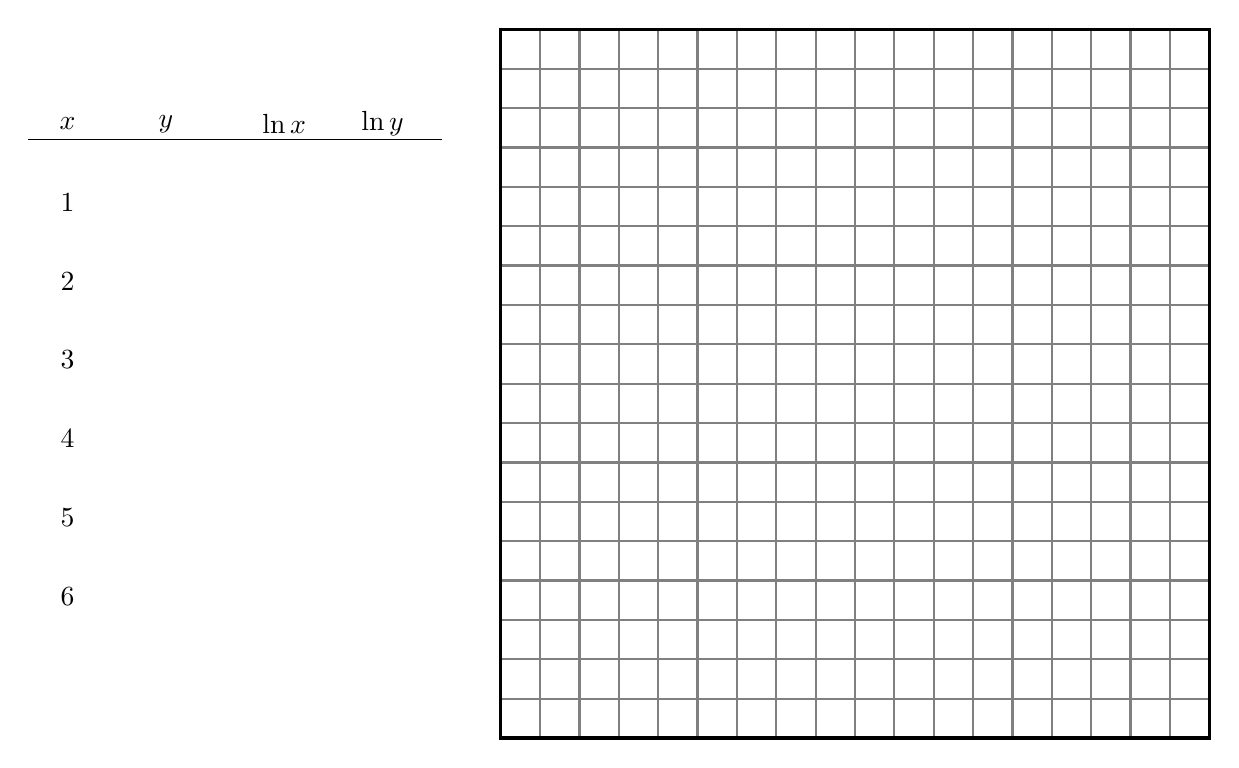
\begin{tikzpicture}
        % Define dimensions
        \def\gridwidth{18}
        \def\gridheight{18}
        \def\spacing{0.5}

        % Draw grid paper on the left
        \begin{scope}[xshift=5.5cm,yshift=0cm]
            % Major grid lines (thicker)
            \foreach \x in {0,1,...,\gridwidth}
                \draw[gray,thick] (\x*\spacing,0) -- (\x*\spacing,\gridheight*\spacing);
            \foreach \y in {0,1,...,\gridheight}
                \draw[gray, thick] (0,\y*\spacing) -- (\gridwidth*\spacing,\y*\spacing);

            % Border around grid
            \draw[black, very thick] (0,0) rectangle (\gridwidth*\spacing,\gridheight*\spacing);
        \end{scope}
        \begin{scope}[yshift=5cm]
            % Table headers
            \node at (0, 2.8) [font=\bfseries] {$x$};
            \node at (1.25, 2.8) [font=\bfseries] {$y$};
            \node at (2.75, 2.8) [font=\bfseries] {$\ln x$};
            \node at (4.0, 2.8) [font=\bfseries] {$\ln y$};

            % Draw horizontal line under headers
             \draw (-0.5, 2.6) -- (4.75, 2.6);

            % Empty rows for data entry
            \foreach \row in {1,...,6}
            {
                \node at (0, 2.8-\row) {\row};
                \node at (1.5, 2.8-\row) {};
             }
        \end{scope}
    \end{tikzpicture}

\end{prelab}

% LAB SECTION
\begin{labsection}

\begin{objective}
    To verify that the electric force between two point charges is directly proportional to the product of their charges and inversely proportional to the square of the distance between them.
\end{objective}

\begin{theory}
    \par Physics in the $18^\text{th}$ century included the study of electric phenomena: how charged objects attract and repel one another.
    In $1785$, Charles-Augustin de Coulomb published the relation we now call Coulomb's Law.
    Given two charges, $q_1$ and $q_2$, separated by a distance, $r$, Coulomb's Law states that the electric force between them is
    \begin{align}\label{eq: Coulomb's Law}
        F = \frac{1}{4\pi\varepsilon_0}\frac{q_1 q_2}{r^2}
    \end{align}
    When we are children, we are told the prefactor is called $k$, but now that you're starting to grow up, we can let you in on the secret.
    The $4\pi$ makes lots of other formulas simpler, and is there because three-dimensional space has that solid angle (remember what the formula for the surface of a sphere is?), while the \textsl{permittivity of free space}, or \textsl{vacuum permittivity}, is in SI units
    \begin{align*}
        \varepsilon_0 = \qty{8.8541878188(14)e-12}{\frac{\coulomb^2\ \second^2}{\kilo\gram\ \meter^3}}.
    \end{align*}
    When plugging stuff in, you can still use what you learned in high school,
    \begin{align*}
        \frac{1}{4\pi\varepsilon_0}\approx \qty{9e9}{\frac{\newton\ \meter^2}{\coulomb^2}}.
    \end{align*}
    The electric force is very powerful compared to gravity.
    In your prelab, you should find that the force in question 2 is on the order of $\qty{1e15}{\newton}$!
    If you could create a force that big to counteract the gravitational force on the Earth's surface, $F=mg$, then you could lift Mt. Everest\footnote{No, seriously, go look up the estimated mass of Mount Everest and calculate its weight.}!

    Verifying Coulomb's law requires some ingenuity since we can't just look at two charged objects moving and know what the force is between them.
    We need something to measure, what we call an \textit{observable}, that can be related to the force in a way that allows us to test equation \ref{eq: Coulomb's Law}.
    To this end, we will use the torsion balance pictured in Figure \ref{fig: torsion balance}.

    \begin{figure*}[ht]
        \centering
        \frame{
\includegraphics[width=0.65\linewidth]{Lab 06: Coulomb's Law/TorsionBalance.png}}
        \caption{The PASCO Model ES-9070 Coulomb Balance.{\color{red} Laraib: can we include a label to the torsion dial in this figure...}}
        \label{fig: torsion balance}
    \end{figure*}

    How does the apparatus work?
    A conductive sphere is mounted on a rod, counterbalanced, and suspended from a thin torsion wire.
    An identical sphere is mounted on a slide assembly so it can be positioned at various distances from the suspended sphere.
    When the spheres have no net charge, the one attached to the wire settles to an equilibrium position and doesn't move.
    Once both spheres are charged, there is an electric force, $F_e$, on each one.

    To charge the spheres, you will use a power supply that can be set to a particular voltage relative to ground, $\Delta V$. Touching the conductive sphere with the charging probe will cause electrons to flow onto it until the two have the same voltage.
    The total charge on the sphere is related to it voltage,
    \begin{align}\label{eq: capacitance}
        q = C\Delta V,
    \end{align}
    where $C$ is the \textit{capacitance} of the conducting sphere, a constant that depends on the sphere's exact size and material composition,
    {\color{red}  which you will learn more about later in the semester (Laraib).}

    The fixed sphere is held in place by the slide assembly, but the other one is free to move, which, in turn, creates a {\sl torque} on the wire\footnote{Don't worry if you don't understand what a torque is yet. You will learn more about torque later in the semester.}. The torque twists the wire, which prefers not to be twisted, and therefore exerts a counter-torque. The more twisted the wire gets, the stronger the counter-torque, until it cancels the first torque and the system settles into a new equilibrium. See Figure \ref{fig: dynamics of torsion balance} for details.

    \begin{figure*}[h]
        \centering
        \frame{
\includegraphics[width=0.8\linewidth]{Lab 06: Coulomb's Law/TorsionExperiment.png}}
        \caption{(Left) The spheres are charged and separated by a fixed distance, $r$, while $d$ is the lever arm for the torque on the wire. (Right) After charging, the wired sphere moves due to the electric force from its twin, twisting the wire. }
        \label{fig: dynamics of torsion balance}
    \end{figure*}

    At this point, the torsion (angular) dial on the Coulomb Balance is used to twist the wire more and pull it back to its original position.
    After this has been done and the system is motionless, the reading on the dial tells you the total twist in the wire, $\Delta \theta$, which is our desired \textit{observable}.
    The strength of the counter torque is described by Hooke's Law,
    \begin{equation}\label{eq: torque 1}
        \tau_+ = -\kappa\Delta \theta,
    \end{equation}
    where $\kappa$ is the {\sl torsion constant} of the wire.
    Meanwhile, the torque due to the electric force is
    \begin{equation}\label{eq: torque 2}
        \tau_- = F_e d,
    \end{equation}
    where $d$ is the {\sl lever arm}, defined as the distance from the wire where the electric force is being applied. The torques cancel in equilibrium, $\tau_++\tau_- = 0$, so combining eqs.~\ref{eq: Coulomb's Law}, \ref{eq: capacitance}, \ref{eq: torque 1}, and \ref{eq: torque 2}, the net twist is
    %
    \begin{align}
        \Delta\theta &=\frac{d}{4\pi\varepsilon_0\kappa}\frac{q_1q_2}{r^2}=\frac{C_1C_2d}{4\pi\varepsilon_0\kappa}\frac{\Delta V_1\Delta V_2}{r^2}\label{eq: observable}
    \end{align}
    %
    Great!
    The prefactor on the right side of equation \ref{eq: observable} is a constant, while the second factor consists of things you can control, the independent variables: $\Delta V_1, \Delta V_2, $ and $r$.
    On the left side of the same equation is the dependent variable, the observable $\Delta \theta$.
    By connecting the electric force to quantities we control and an observable, it is possible to test the veracity of Coulomb's Law, {\color{red} Laraib: where $\Delta\theta$ acts as a proxy for the force $F$, while $\Delta V_1$ and $\Delta V_2$ serve as proxies for the charges $Q_1$ and $Q_2$.}

    In {\bf Experiment 1}, every variable in equation \ref{eq: observable} will be held constant except for $r$. This will test the proportionality relation
    %
    \begin{equation*}
        \Delta \theta\propto \frac{1}{r^2}.
    \end{equation*}
    %
    In {\bf Experiment 2}, every variable will be kept constant except $q_2=C_2\Delta V_2$, testing the proportionality
    %
    \begin{equation*}
        \Delta \theta\propto q_2\propto \Delta V_2.
    \end{equation*}
    %
    In both experiments, you will charge the spheres up to a given voltage. Note that your bodies, the air, and other objects in the lab have charges on them that may interfere with measurements or cause the charges on the spheres to leak into the environment.
\end{theory}

\begin{equipment}
\item PASCO Model ES-9070 Torsion Balance (see Fig.~\ref{fig: torsion balance})
\item Two conducting spheres of radius $a=\qty{1.9}{\centi\meter}$
\item Power supply with a power cord
\item {\color{red}\textbf{Red}} and \textbf{Black} wires with probes
\end{equipment}

\begin{experiment}
\subsection*{Tips for Accurate Results}
\begin{itemize}
    \item To minimize the influence of any static charge on your body, stand directly behind the balance and as far away as possible.
    \item Avoid synthetic fabrics since they tend to acquire large static charges.
    Short-sleeve cotton shirts are best. Attaching a grounding wire to the experimenter further reduces the impact of static charges.
    \item Turn the power supply on, charge the spheres, and immediately turn the power supply off.
    The large voltages can affect the torsion balance.
    \item While charging, hold the probe near the end of the handle so that your hand is as far from the sphere as possible to minimize bioelectric effects.
    \item Avoid handling the spheres as much as possible, and wipe them with alcohol {\color{red} Laraib: We don't really do this during the lab, so either can remove this or start doing that...} after touching their surfaces. Even trace amounts of oils from your skin will alter their capacitance.
    \item Perform the measurements as quickly as possible after charging the spheres to minimize charge leakage.
    \item Recharge the spheres before each measurement.
\end{itemize}

\subsection*{Experiment 1: Varying $r$}\label{subsec: experiment 1}
\begin{enumerate}
    \item Touch the spheres with the grounding probe to ensure they are fully discharged. Move the sliding sphere as far as possible from the suspended sphere.
    Set the torsion dial to \ang{0}.
    Zero the torsion balance by rotating the bottom torsion wire retainer until the pendulum is at the zero displacement position.
    \item Ground both spheres again with the grounding probe.
    Position the slide arm to $2a=\qty{3.8}{\centi\meter}$, the diameter of a sphere.
    Loosen the thumbscrew on the rod supporting the sliding sphere and move it until the sliding sphere is just touching the suspended sphere.
    Do not push the suspended sphere causing it to rotate.
    Tighten the thumbscrew.
    \item Move the sliding sphere as far away as possible from the suspended sphere.
    Use the charging probe to charge each sphere to a potential of \qty{6}{\kilo\volt}.
    \item Move the sliding arm to $r=\qty{20}{\centi\meter}$.
    Adjust the torsion dial to bring the pendulum back to the zero position.
    Record this first measurement of $\Delta\theta$ in the first row of Table~\ref{tab: measurement 1 data}.
    \item Repeat steps 3-4 until the results you're getting fall within $\pm\qty{1}{\degree}$ of each other, remembering to record every measurement of $\Delta\theta$ in Table~\ref{tab: measurement 1 data}.
    \item Repeat steps 3-5 for other values of $r$ at \qty{14}{\centi\meter}, \qty{10}{\centi\meter}, \qty{9}{\centi\meter}, \qty{8}{\centi\meter}, \qty{7}{\centi\meter}, \qty{6}{\centi\meter}, and \qty{5}{\centi\meter} {\color{red} Laraib: suggestion: these are measurements for 8 r's..i think we can do with 6}.
\end{enumerate}

\subsection*{Experiment 2: Varying $q_2$}\label{subsec: experiment 2}
\begin{enumerate}
    \item Same as Experiment 1.
    \item Same as Experiment 1.
    \item Same as Experiment 1.
    \item Move the sliding arm to \qty{8}{\centi\meter}.
    Adjust the torsion dial to bring the pendulum back to the zero position.
    Record $\Delta\theta$ in Table~\ref{tab: measurement 2 data}.
    \item Repeat steps 3-4 at least 5 times, until successive measurements are falling within $\pm$\qty{1}{\degree} of each other.
    Don't forget to record everything!
    \item Repeat steps 3-5 but charging the sliding sphere to different potentials, namely \qty{5}{\kilo\volt}, \qty{4}{\kilo\volt}, \qty{3}{\kilo\volt}, \qty{2}{\kilo\volt}, and \qty{1}{\kilo\volt}, while keeping the suspended sphere at \qty{6}{\kilo\volt}.
\end{enumerate}

\end{experiment}

\end{labsection}

% POSTLAB SECTION
\begin{postlab}

\question[4] \textbf{Measurement 1: Force vs.\ Separation.}

Coulomb's Law applies to point charges, but we use spheres of radius $a$. When the spheres are far apart such that $r\gg a$, they behave like point charges because the charge on each is spread out more or less uniformly. But when the spheres are close together such that $r\approx a$, the charge on each sphere bunches up, leading to non-pointlike behavior. In a more advanced class, you may learn how to calculate this effect, but for now, it suffices to know that the corrected observable is
%
\begin{align}\label{eq: observable corrected}
    \Delta \theta_c &= \frac{\Delta \theta}{\beta}, &
    &\text{where} &
    \beta &= 1-4\left(\frac{a}{r}\right)^3
\end{align}
%
is the correction factor. In Table~\ref{tab: measurement 1 data}, write your measurements of $\Delta\theta$ for each separation $r$ and compute the mean of your $N$ measurements:
%
\begin{equation}\label{eq: mean angle}
    \overline{\Delta\theta} = \frac{1}{N}\sum_{i=1}^N \Delta\theta_i.
\end{equation}
%
Then compute the correction factor $\beta$ and the corrected mean twist angle $\overline{\Delta\theta}_c$ using eq.~\ref{eq: observable corrected}. Finally, for each row and separation $r$, tabulate $1/r^2$, $\ln{(r/a)}$, and $\ln{\overline{\Delta\theta}_c}$. You will plot the final two columns on the next page.

\begin{table}[ht]
    \captionsetup{font=normalsize, textfont=bf}
    \centering
    \caption{Measurement 1 Data}
    \renewcommand{\arraystretch}{2.0}
    \begin{tabular}{|c|>{\centering}p{4.5cm}|>{\centering}p{1.2cm}|>{\centering}p{1cm}|>{\centering}p{1.2cm}|>{\centering}p{1cm}|>{\centering}p{1.2cm}|c|}
        \hline
        \rowcolor{EverButter}
        $r$ [cm] & $\Delta\theta$ & $\overline{\Delta\theta}$ [$^\circ$] & $\beta$ & $\overline{\Delta\theta}_c$ [$^\circ$] & $1/r^2$ & $\ln{(r/a)}$ & $\ln{(\overline{\Delta\theta}_c)}$
        \\
        \hline
        20 & & & & & & &
        \\
        \hline
        14 & & & & & & &
        \\
        \hline
        10 & & & & & & &
        \\
        \hline
        9 & & & & & & &
        \\
        \hline
        8 & & & & & & &
        \\
        \hline
        7 & & & & & & &
        \\
        \hline
        6 & & & & & & &
        \\
        \hline
        5 & & & & & & &
        \\
        \hline
    \end{tabular}
    \renewcommand{\arraystretch}{1.0}
    \label{tab: measurement 1 data}
\end{table}

\question[4] \textbf{Measurement 2: Force vs.\ Charge.}

Fill in Table~\ref{tab: measurement 2 data} with your measurements from Experiment 2.

\begin{table}[ht]
    \captionsetup{font=normalsize, textfont=bf}
    \centering
    \caption{Measurement 2 Data}
    \renewcommand{\arraystretch}{2.0}
    \begin{tabular}{|c|>{\centering}p{4.5cm}|>{\centering}p{1.2cm}|>{\centering}p{1cm}|>{\centering}p{1.2cm}|>{\centering}p{1.2cm}|c|}
        \hline
        \rowcolor{EverButter}
        $\Delta V_2$ [kV] & $\Delta\theta$ & $\overline{\Delta\theta}$ [$^\circ$] & $\beta$ & $\overline{\Delta\theta}_c$ [$^\circ$] & $\ln{(\overline{\Delta\theta}_c)}$ & $\ln{(\Delta V_2/\qty{1}{\kilo\volt})}$
        \\
        \hline
        6 & & & & & &
        \\
        \hline
        5 & & & & & &
        \\
        \hline
        4 & & & & & &
        \\
        \hline
        3 & & & & & &
        \\
        \hline
        2 & & & & & &
        \\
        \hline
        1 & & & & & &
        \\
        \hline
    \end{tabular}
    \renewcommand{\arraystretch}{1.0}
    \label{tab: measurement 2 data}
\end{table}

\newpage

\question[3] Make a scatter plot of $\ln{(\overline{\Delta\theta}_c)}$ vs. $\ln{(r/a)}$ with the independent variable on the horizontal axis and the dependent variable on the vertical axis. Label your axes.
    \begin{center}
        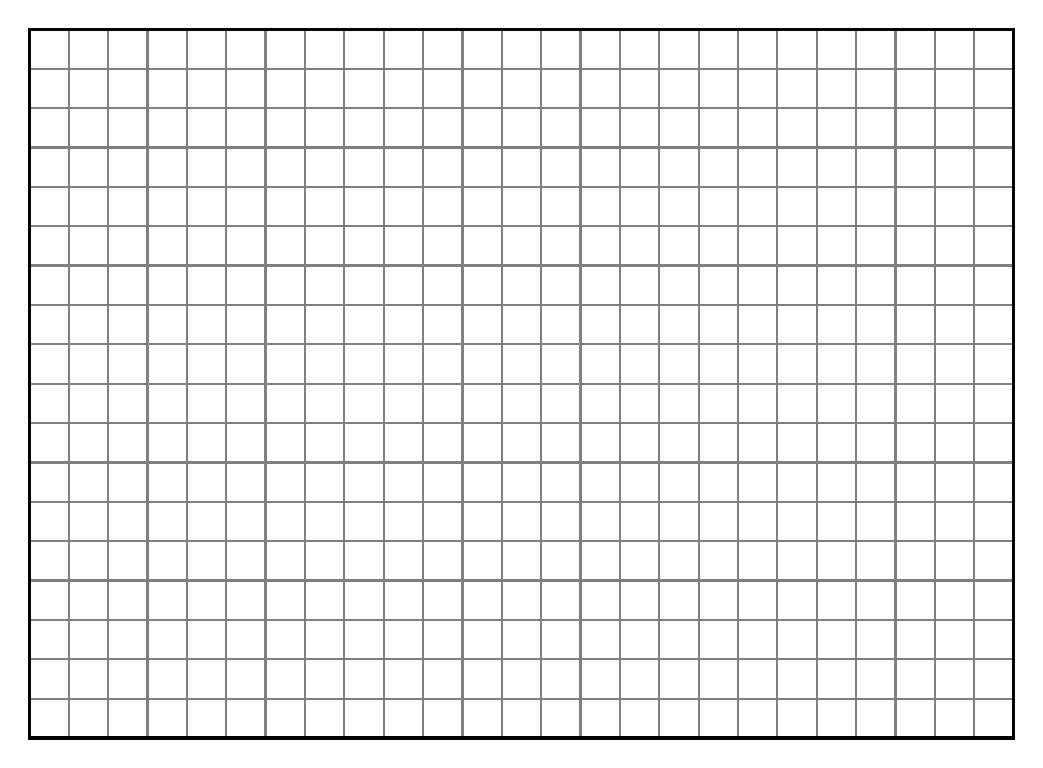
\begin{tikzpicture}
            % Define dimensions
            \def\gridwidth{25}
            \def\gridheight{18}
            \def\spacing{0.5}
            % Draw grid paper on the left
            \begin{scope}[xshift=0cm,yshift=0cm]
                % Major grid lines (thicker)
                \foreach \x in {0,1,...,\gridwidth}
                    \draw[gray,thick] (\x*\spacing,0) -- (\x*\spacing,\gridheight*\spacing);
                \foreach \y in {0,1,...,\gridheight}
                    \draw[gray, thick] (0,\y*\spacing) -- (\gridwidth*\spacing,\y*\spacing);
                \draw[black, very thick] (0,0) rectangle (\gridwidth*\spacing,\gridheight*\spacing);
            \end{scope}
        \end{tikzpicture}
    \end{center}

\question[3] Make a scatter plot of $\ln{(\overline{\Delta\theta}_c)}$ vs. $\ln(\Delta V_2/1\text{kV})$ with the independent variable on the horizontal axis and the dependent variable on the vertical axis. Label your axes.
\begin{center}
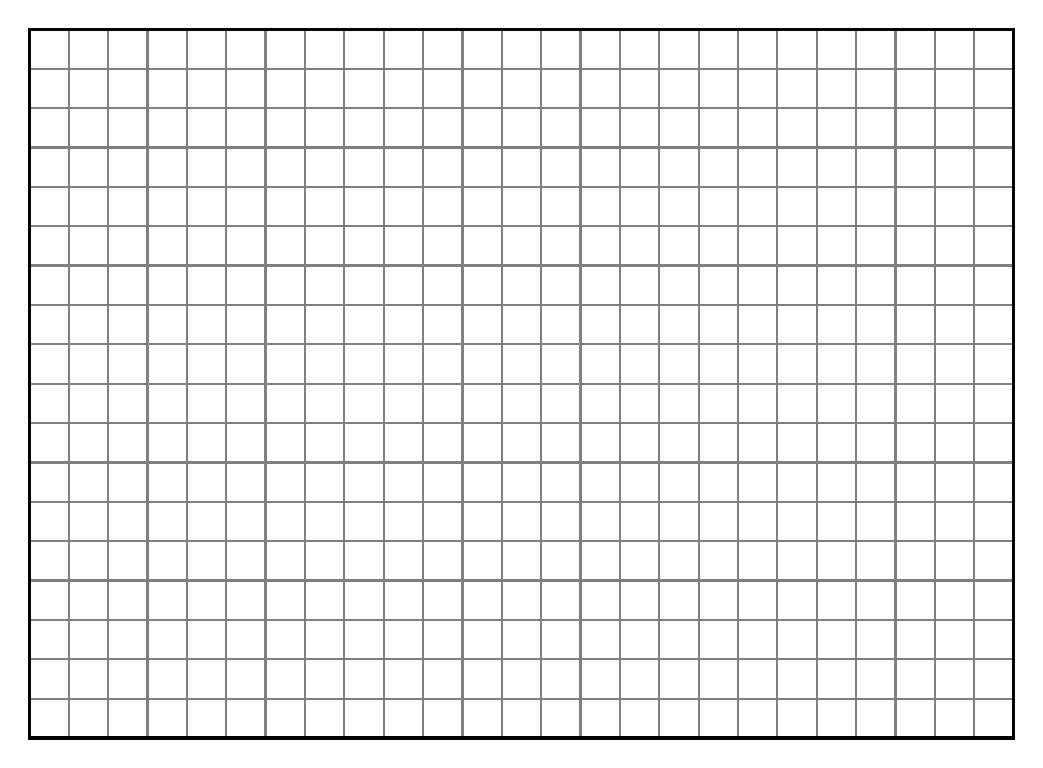
\begin{tikzpicture}
\def\gridwidth{25}
\def\gridheight{18}
\def\spacing{0.5}
            \begin{scope}[xshift=0cm,yshift=0cm]
                \foreach \x in {0,1,...,\gridwidth}
                \draw[gray,thick] (\x*\spacing,0) -- (\x*\spacing,\gridheight*\spacing);
                \foreach \y in {0,1,...,\gridheight}
                \draw[gray, thick] (0,\y*\spacing) -- (\gridwidth*\spacing,\y*\spacing);
                \draw[black, very thick] (0,0) rectangle (\gridwidth*\spacing,\gridheight*\spacing);
            \end{scope}
        \end{tikzpicture}
    \end{center}

\newpage

\question[3] For both graphs add a dashed line that fits the data well.
        Use the plots to estimate the $y-$intercept and slope of each line, and write down the equation of the line for each {\color{red} Laraib: in the form y=mx+b, where m is the slope and b is the y-intercept..is this what you mean?}.
        \begin{solution}[150pt]
        \end{solution}

\question[3] If Coulomb's Law holds, what slope do you expect each line to have?
        Is this what you measured?
        What is the reason for the deviation? {\color{red} Laraib: i.e. provide possible sources of error in your experiment?}
        {\color{red} Laraib: we could possibly switch Question 4 to a qualitative analysis rather than a quantitative measurement, like: Analyze the best-fit lines to both your plots. What mathematical
        relationship exists between $\ln{(\overline{\Delta\theta}_c)}$ and $\ln{(r/a)}$, and $\ln{(\overline{\Delta\theta}_c)}$ and $\ln(\Delta V_2/1)$? Does this match with Coulomb's law?}
        \begin{solution}[150pt]
        \end{solution}

{\color{red} Laraib: I think we need a picture of the torsion dial: one with alignment with 0 and one with a non-zero angular reading - a lot of students get confused about how to use the torsion dial to measure the angle, and i think a figure for that would be helpful}.

\end{postlab}

\end{document}
